The IDDR implementation uses the \texttt{Linux kernel 3.5.0} for both application domain and driver domain. We test the IDDR system it with Arch Linux on \texttt{x86\_64} platform. The specification of the system used for evaluation is presented in the table~\ref{tab:config}. 

\begin{table}
\caption{Hardware specifications of the system}
\begin{center}
\begin{tabular}{ll}
  \hline
  \label{tab:config}
  System Parameter & Configuration \\
  \hline
  Processor & 1 X Quad-code AMD Opteron(tm) Processor 2380, 2.49 Ghz \\
  Number of cores & 4 per processor \\
  Hyperthreading & OFF \\
  %Turbo boost & ?? \\
  L1 L2 cache & 64K/512K per core \\
  L3 cache & 6144K \\
  Main memory & 16Gb \\
  Storage & SATA, HDD ??RPM \\
  \hline 
\end{tabular}
\end{center}
\end{table}

\section{Goals}
\label{sec:goals}
The goals of the IDDR system evaluation are:
%\begin{itemize} 
\begin{enumerate}
\item Comparison of the Xen's isolated driver domain with the base IDDR system.
\\[3mm]
The goal of this thesis is to explore the performance improvement opportunity in the Xen's isolated driver domain and implement it. However, the source code for the isolated driver domain is not available in the open source Xen hypervisor. As a result, we re-implement the isolated driver domain and call it the base Isolated Device Driver (IDDR) system. We implement the spinlock based communication channel over the base IDDR system and refer to it as the new IDDR system.
\\[3mm]
In order to prove the performance improvement of the new IDDR system over the base IDDR system and the Xen's isolated driver domain, it is necessary to compare the performance of the Xen's isolated driver domain with the base IDDR system. The Xen's isolated driver domain follows split device driver architecture, which has gone over decade for the performance testing. We achieve this evaluation goal by comparing the performance of the base IDDR system with the Xen split device driver. The comparison of both shows that the performance of the IDDR system matches the performance of the Xen's isolated driver domain. Hence, proves that our implementation provides a suitable baseline for the performance improvement.

\item an evaluation of IDDR performance improvement over base IDDR system,
\\[3mm] 
The second goal of the evaluation is to prove that the spinlock based communication channel improves the performance of the inter-domain communication and hence the IDDR system.
\\[3mm]
We achieve this evaluation goal by comparing the performance of the base IDDR system with the new IDDR system. The comparison shows that the new IDDR system performs better than the base IDDR system and the Xen's isolated driver domain.
%\end{itemize}
\end{enumerate}

\section{Methodology}
In order to measure the performance of the system, we run performance tests against the variety of block devices. In a Linux system, a loop device is a device that makes a file accessible as a block device. A ramdisk is a block of a memory, which acts as a disk drive. In order to cover a variety of the devices we use block devices such as SATA disk, ramdisk and loop device for the performance testing.
\\[3mm]
For the performance tests, we format the block device with the ext2 file system, and run the fileIO SysBench benchmark~\cite{sysbench} on it. SysBench is a multi-threaded benchmark tool for evaluating a system. It evaluates the system performance without installing a database or without setting up complex database benchmarks. Sysbench benchmark has different test modes. FileIO is one of the test mode which can be used to produce various file I/O workloads. SysBench can run a specified number of threads by executing all requests in parallel. Sysbench benchmark in fileIO test mode generates 128 files with \texttt{1Gb} of total data and performs random reads, random writes and mix of random read-writes with a block size of \texttt{16Kb}. 

\section{The Xen Split Device Driver vs The Base IDDR System}
As per our first goal of evaluation mentioned in Section~\ref{sec:goals}, we compare the base IDDR with the Xen split device driver. In this comparison, we show that the performance of the base IDDR system matches the Xen's isolated driver domain. This verifies the baseline performance of the IDDR system.

\subsection{Experimental Setup}

\subsubsection*{The Xen Split Device Driver}
We create a ramdisk in the domain 0. The guest domain (domain U) is configured such that the ramdisk uses a split device driver and it is available in the guest domain. We do a similar setup for the loop device and the SATA disk. For example, in case of loop device, we create a loop device in domain 0 and then configure the guest domain to use the loop device as a disk. In case of SATA disk, we configure the guest domain to use SATA disk as a secondary disk. We format and mount the disk in the guest domain with the ext2 file system. Sysbench benchmark is run on the mounted partition as explained in section~\ref{sec:goals}.

\subsubsection*{The Base IDDR System}
In a Xen hypervisor, the domain 0 always runs as a PV guest and in our setup we run the domain U as a HVM guest.
\\[3mm] 
In Xen, paravirtualized guest is a guest which is aware of the VMM and require special ported kernel to run efficiently without emulation or virtual emulated hardware. Paravirtualization does not require virtualization extensions from the host CPU. 
\\[3mm]
On the other hand, fully virtualized or hardware virtual machine (HVM) guest require CPU virtualization extensions such as Intel VT, AMD-V. The Xen uses modified version of Qemu to emulate hardware for HVM guests. CPU virtualization extensions are used to boost performance of the emulation. A fully virtualized guest does not require special kernel. In order to boost the performance, fully virtualized HVM guest uses special paravirtual device drivers and bypasses the emulation for disk and network IO.
\\[3mm]
A HVM guest is expected to have less syscall overhead and faster memory bandwidth than a PV guest. In the Xen split device driver setup, the backend device driver runs in the domain 0 and the frontend device driver runs in a domain U. In order to compare the Xen split device driver and the base IDDR system, it is necessary to run the backend driver of the IDDR system in the domain 0 and the frontend driver of the IDDR system in the domain U.
\\[3mm]
We insert a ramdisk and the base IDDR system's frontend module in the domain 0. The base IDDR system's backend module is inserted in the guest domain (domain U). We format and mount the ramdisk with ext2 file system and sysbench benchmark is run on it.  
\\[3mm]
Similar setup is used for a loop device and a SATA disk.
\subsubsection*{Comparison}
Figure~\ref{fig:iddrvsxen-ramdisk-rdwr} shows the performance of random reads-writes on a ramdisk, and Figure~\ref{fig:iddrvsxen-loop-rd} shows the performance of random reads on a loop device. Both systems provide roughly similar performance. The figures show that the performance of the IDDR matches the performance of the Xen's isolated driver domain. Therefore, our implementation of the Xen's isolated driver domain provides suitable baseline for the performance improvement.
\begin{figure}[!ht]
\centering
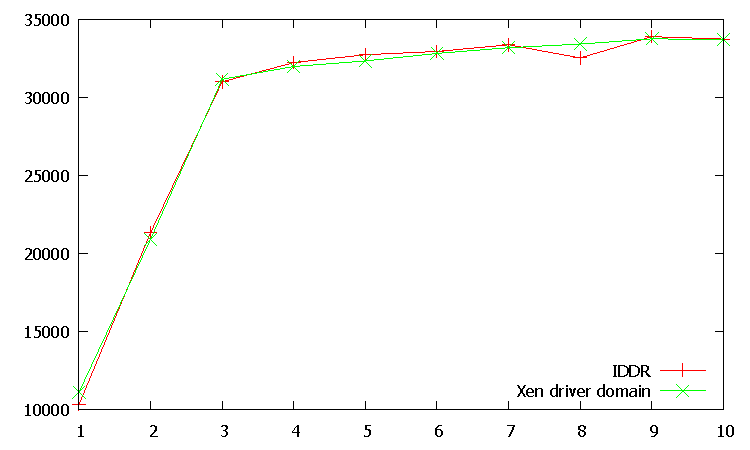
\includegraphics[scale=1]{iddrvsxen-ramdisk-rdwr}
\caption{The base IDDR system vs The Xen split device driver (ramdisk)}
\label{fig:iddrvsxen-ramdisk-rdwr}
\end{figure}
\begin{figure}[!ht]
\centering
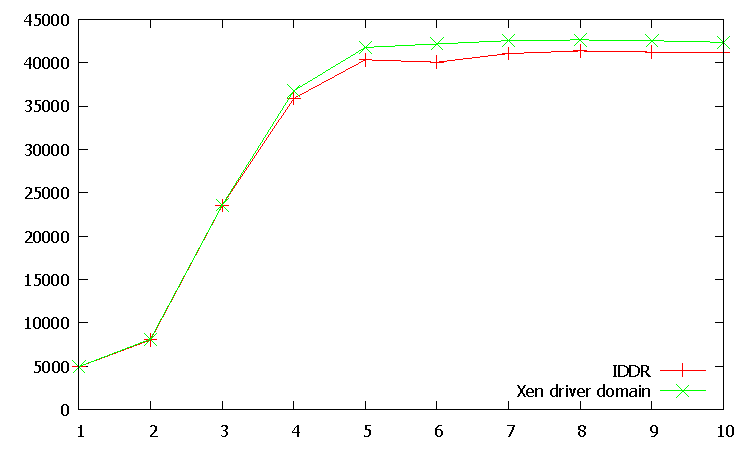
\includegraphics[scale=1]{iddrvsxen-loop-rd}
\caption{The base IDDR system vs The Xen split device driver (loop device)}
\label{fig:iddrvsxen-loop-rd}
\end{figure}

\section{The Base IDDR System vs The New IDDR System}
We measure and compare the performance of the base IDDR system with the new IDDR system. We run the fileIO sysbench benchmark with random reads, random writes and mixed random reads-writes. 
\subsection*{Experimental Setup}
In the base IDDR system and the new IDDR system, the domain 0 is an application domain, and a domain U is the driver domain. A ramdisk is created in the driver domain. The backend driver is inserted in the driver domain and the frontend driver is inserted in the application domain. The disk is formatted and mounted with ext2 file system in the application domain. Sysbench benchmark is run on the mounted partition. 
\\[3mm]
For loop device a similar setup is used, we create a loop device in a driver domain, and insert the backend driver in the driver domain. The frontend driver is inserted in the application domain. For a SATA disk, we pass-through the SATA disk to the driver domain, so that the driver domain can directly access the SATA disk. 
\subsubsection*{Comparison}
Figure~\ref{fig:threadvsspinram} compares the performance of the base IDDR and the new IDDR with random reads-writes on a ramdisk. Figure~\ref{fig:threadvsspinloop} compares the performance of the base IDDR and the new IDDR with random reads on a loop device. Both figures show that the new IDDR system implementation with spinlock performs better than the base IDDR implementation. 
\begin{figure}[!ht]
\centering
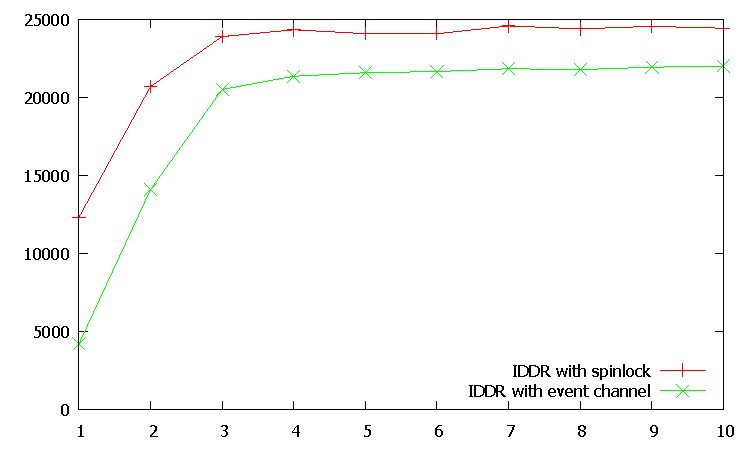
\includegraphics[scale=1]{threadvsspinram}
\caption{The base IDDR system vs the new IDDR system (ramdisk)}
\label{fig:threadvsspinram}
\end{figure}
\begin{figure}[!ht]
\centering
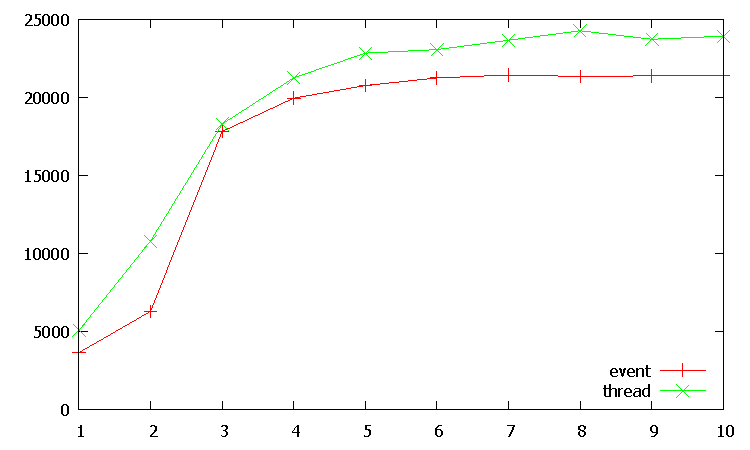
\includegraphics[scale=1]{threadvsspinloop}
\caption{The base IDDR system vs the new IDDR system (loop device)}
\label{fig:threadvsspinloop}
\end{figure}


% ref
\ifbool{toShowBibliography}{\bibliography{references}}{}